% ===========================================================================
% Section 5: Results — Incremental Port Load Test
% ===========================================================================
\section{Results: Incremental Port Load Test}
\label{sec:results}

This section presents the results of Test~1 (Section~\ref{sec:test-incremental-port-load}).
We first present per-device power and throughput profiles, then analyze the data in the context of the research questions addressed by this test.

% ---------------------------------------------------------------------------
\subsection{Per-Device Results}
\label{sec:per-device-results}
% ---------------------------------------------------------------------------

% ===== FRITZBOX =====
\subsubsection{Fritzbox 7530}
\label{sec:results-fritzbox}

\begin{figure}[H]
    \centering
    \begin{tikzpicture}
        \begin{axis}[
            width=0.95\linewidth,
            height=7cm,
            xlabel={Elapsed Time (s)},
            ylabel={Power (mW)},
            xmin=0, xmax=6600,
            ymin=4200, ymax=5800,
            grid=major,
            grid style={gray!30},
            legend pos=north west,
            legend style={font=\small},
            title={Fritzbox 7530 --- Power Consumption Over Time},
            % Phase boundary lines
            extra x ticks={600, 1800, 3000, 4200, 5400},
            extra x tick labels={},
            extra x tick style={grid=major, grid style={dashed, red!50, line width=0.8pt}},
        ]
            \addplot[blue, very thin, each nth point=1] table[col sep=comma, x=ElapsedSeconds, y=PowerMW] {data/fritzbox_data.csv};
            \addlegendentry{Power}

            % Phase labels
            \node[font=\tiny, rotate=90, anchor=south] at (axis cs:300,5700) {Idle};
            \node[font=\tiny, rotate=90, anchor=south] at (axis cs:1200,5700) {1 Port};
            \node[font=\tiny, rotate=90, anchor=south] at (axis cs:2400,5700) {2 Ports};
            \node[font=\tiny, rotate=90, anchor=south] at (axis cs:3600,5700) {3 Ports};
            \node[font=\tiny, rotate=90, anchor=south] at (axis cs:4800,5700) {4 Ports};
            \node[font=\tiny, rotate=90, anchor=south] at (axis cs:6000,5700) {Post};

            % Baseline reference
            \draw[dashed, gray, thin] (axis cs:0,4432) -- (axis cs:6600,4432);
        \end{axis}
    \end{tikzpicture}
    \caption{Fritzbox 7530: Power consumption over time. Dashed vertical lines mark phase transitions (600\,s, 1800\,s, 3000\,s, 4200\,s, 5400\,s). Horizontal dashed line indicates idle baseline (4432\,mW).}
    \label{fig:fritzbox_power}
\end{figure}

\begin{figure}[H]
    \centering
    \begin{tikzpicture}
        \begin{axis}[
            width=0.95\linewidth,
            height=7cm,
            xlabel={Elapsed Time (s)},
            ylabel={Throughput (Mbps)},
            xmin=0, xmax=6600,
            ymin=0, ymax=4500,
            grid=major,
            grid style={gray!30},
            legend pos=north west,
            legend style={font=\small},
            title={Fritzbox 7530 --- Aggregate Throughput Over Time},
            extra x ticks={600, 1800, 3000, 4200, 5400},
            extra x tick labels={},
            extra x tick style={grid=major, grid style={dashed, red!50, line width=0.8pt}},
        ]
            \addplot[teal, very thin, each nth point=1] table[col sep=comma, x=ElapsedSeconds, y=ThroughputTotalMbps] {data/fritzbox_data.csv};
            \addlegendentry{Throughput}
        \end{axis}
    \end{tikzpicture}
    \caption{Fritzbox 7530: Aggregate throughput. Note the significant throughput spikes at phase transitions and the decline in total throughput at 3--4~ports due to CPU saturation.}
    \label{fig:fritzbox_throughput}
\end{figure}

The Fritzbox~7530 showed a clear CPU bottleneck effect: total throughput actually \emph{decreased} when moving from 2 to 3 and 4~ports (from $\sim$2483\,Mbps to $\sim$1827\,Mbps aggregate), while power remained relatively flat around 5000--5130\,mW.
The idle baseline averaged 4432\,mW ($\pm$19\,mW).
The post-test baseline was notably higher and more variable (4531\,mW $\pm$223\,mW), suggesting thermal effects or delayed power state recovery.

% ===== HUAWEI =====
\subsubsection{Huawei EchoLife EG8245W5-8T}
\label{sec:results-huawei}

\begin{figure}[H]
    \centering
    \begin{tikzpicture}
        \begin{axis}[
            width=0.95\linewidth,
            height=7cm,
            xlabel={Elapsed Time (s)},
            ylabel={Power (mW)},
            xmin=0, xmax=6600,
            ymin=8600, ymax=9800,
            grid=major,
            grid style={gray!30},
            legend pos=north west,
            legend style={font=\small},
            title={Huawei EG8245W5-8T --- Power Consumption Over Time},
            extra x ticks={600, 1800, 3000, 4200, 5400},
            extra x tick labels={},
            extra x tick style={grid=major, grid style={dashed, red!50, line width=0.8pt}},
        ]
            \addplot[blue, very thin, each nth point=1] table[col sep=comma, x=ElapsedSeconds, y=PowerMW] {data/huawei_data.csv};
            \addlegendentry{Power}
            \draw[dashed, gray, thin] (axis cs:0,8962) -- (axis cs:6600,8962);

            \node[font=\tiny, rotate=90, anchor=south] at (axis cs:300,9700) {Idle};
            \node[font=\tiny, rotate=90, anchor=south] at (axis cs:1200,9700) {1 Port};
            \node[font=\tiny, rotate=90, anchor=south] at (axis cs:2400,9700) {2 Ports};
            \node[font=\tiny, rotate=90, anchor=south] at (axis cs:3600,9700) {3 Ports};
            \node[font=\tiny, rotate=90, anchor=south] at (axis cs:4800,9700) {4 Ports};
            \node[font=\tiny, rotate=90, anchor=south] at (axis cs:6000,9700) {Post};
        \end{axis}
    \end{tikzpicture}
    \caption{Huawei EG8245W5-8T: Power consumption over time. The power profile is very flat, with only $\sim$550\,mW total increase from idle to 4-port full load.}
    \label{fig:huawei_power}
\end{figure}

The Huawei showed the most efficient scaling behavior.
Idle power averaged 8962\,mW, rising monotonically to 9510\,mW under full 4-port load---an increase of only 548\,mW (+6.1\%) while achieving $\sim$3815\,Mbps aggregate throughput (near the theoretical 4$\times$1\,Gbps maximum).
The post-test baseline returned cleanly to 8986\,mW, within 24\,mW of the pre-test value.

% ===== ASUS =====
\subsubsection{Asus RT-AX68U}
\label{sec:results-asus}

\begin{figure}[H]
    \centering
    \begin{tikzpicture}
        \begin{axis}[
            width=0.95\linewidth,
            height=7cm,
            xlabel={Elapsed Time (s)},
            ylabel={Power (mW)},
            xmin=0, xmax=6600,
            ymin=7900, ymax=9500,
            grid=major,
            grid style={gray!30},
            legend pos=north west,
            legend style={font=\small},
            title={Asus RT-AX68U --- Power Consumption Over Time},
            extra x ticks={600, 1800, 3000, 4200, 5400},
            extra x tick labels={},
            extra x tick style={grid=major, grid style={dashed, red!50, line width=0.8pt}},
        ]
            \addplot[blue, very thin, each nth point=1] table[col sep=comma, x=ElapsedSeconds, y=PowerMW] {data/asus_data.csv};
            \addlegendentry{Power}
            \draw[dashed, gray, thin] (axis cs:0,8226) -- (axis cs:6600,8226);

            \node[font=\tiny, rotate=90, anchor=south] at (axis cs:300,9400) {Idle};
            \node[font=\tiny, rotate=90, anchor=south] at (axis cs:1200,9400) {1 Port};
            \node[font=\tiny, rotate=90, anchor=south] at (axis cs:2400,9400) {2 Ports};
            \node[font=\tiny, rotate=90, anchor=south] at (axis cs:3600,9400) {3 Ports};
            \node[font=\tiny, rotate=90, anchor=south] at (axis cs:4800,9400) {4 Ports};
            \node[font=\tiny, rotate=90, anchor=south] at (axis cs:6000,9400) {Post};
        \end{axis}
    \end{tikzpicture}
    \caption{Asus RT-AX68U: Power consumption over time. Shows a clear step-wise increase with each additional loaded port.}
    \label{fig:asus_power}
\end{figure}

The Asus RT-AX68U demonstrated excellent throughput scaling (achieving $\sim$3816\,Mbps at 4~ports) with a moderate power increase from 8226\,mW idle to 8933\,mW at full load (+707\,mW, +8.6\%).
The power increase per additional port was approximately 175\,mW on average.
Post-test recovery was prompt, returning to 8257\,mW ($+$31\,mW from pre-test).

% ===== ALCATEL =====
\subsubsection{Alcatel HH40V}
\label{sec:results-alcatel}

\begin{figure}[H]
    \centering
    \begin{tikzpicture}
        \begin{axis}[
            width=0.95\linewidth,
            height=7cm,
            xlabel={Elapsed Time (s)},
            ylabel={Power (mW)},
            xmin=0, xmax=4200,
            ymin=1600, ymax=2300,
            grid=major,
            grid style={gray!30},
            legend pos=north west,
            legend style={font=\small},
            title={Alcatel HH40V --- Power Consumption Over Time},
            extra x ticks={600, 1800, 3000},
            extra x tick labels={},
            extra x tick style={grid=major, grid style={dashed, red!50, line width=0.8pt}},
        ]
            \addplot[blue, very thin, each nth point=1] table[col sep=comma, x=ElapsedSeconds, y=PowerMW] {data/alcatel_data.csv};
            \addlegendentry{Power}
            \draw[dashed, gray, thin] (axis cs:0,1854) -- (axis cs:4200,1854);

            \node[font=\tiny, rotate=90, anchor=south] at (axis cs:300,2250) {Idle};
            \node[font=\tiny, rotate=90, anchor=south] at (axis cs:1200,2250) {1 Port};
            \node[font=\tiny, rotate=90, anchor=south] at (axis cs:2400,2250) {2 Ports};
            \node[font=\tiny, rotate=90, anchor=south] at (axis cs:3600,2250) {Post};
        \end{axis}
    \end{tikzpicture}
    \caption{Alcatel HH40V: Power consumption over time. Only 2 ports available (100\,Mbps each). Despite low absolute power, the relative increase per port is significant.}
    \label{fig:alcatel_power}
\end{figure}

The Alcatel~HH40V, with only two 100\,Mbps ports, showed the lowest absolute power consumption (idle: 1854\,mW).
Under full 2-port load, power rose to 2076\,mW ($+$222\,mW, $+$12.0\%).
Throughput reached $\sim$257\,Mbps total across both ports (close to the theoretical 200\,Mbps maximum; the slightly higher measured value likely includes transient measurement artifacts from the 5-second polling window).

% ---------------------------------------------------------------------------
\subsection{Cross-Device Comparison}
\label{sec:cross-device-comparison}
% ---------------------------------------------------------------------------

% ===== RQ1: Power vs Port Count =====
\subsubsection{RQ1: Power Consumption vs.\ Number of Active Ports}
\label{sec:rq1-results}

Table~\ref{tab:power-per-phase} summarizes the average power consumption during each load phase for all four devices.

\begin{table}[H]
    \centering
    \caption{Average power consumption (mW) by load phase for each device. $\Delta$ columns show the increase relative to the idle baseline.}
    \label{tab:power-per-phase}
    \footnotesize
    \begin{tabular}{l r r r r r r r r}
        \toprule
        \textbf{Device} & \textbf{Idle} & \textbf{1\,Pt} & $\Delta$ & \textbf{2\,Pt} & $\Delta$ & \textbf{3\,Pt} & \textbf{4\,Pt} & $\Delta_{\text{max}}$ \\
        \midrule
        Fritzbox 7530   & 4432 & 4800 & +368  & 5055 & +623  & 5040 & 5132 & +700 (+15.8\%) \\
        Huawei EG8245W5 & 8962 & 9231 & +269  & 9409 & +447  & 9494 & 9510 & +548 (+6.1\%) \\
        Asus RT-AX68U   & 8226 & 8726 & +500  & 8806 & +580  & 8852 & 8933 & +707 (+8.6\%) \\
        Alcatel HH40V   & 1854 & 1977 & +123  & 2076 & +222  & ---  & ---  & +222 (+12.0\%) \\
        \bottomrule
    \end{tabular}
\end{table}

\begin{figure}[H]
    \centering
    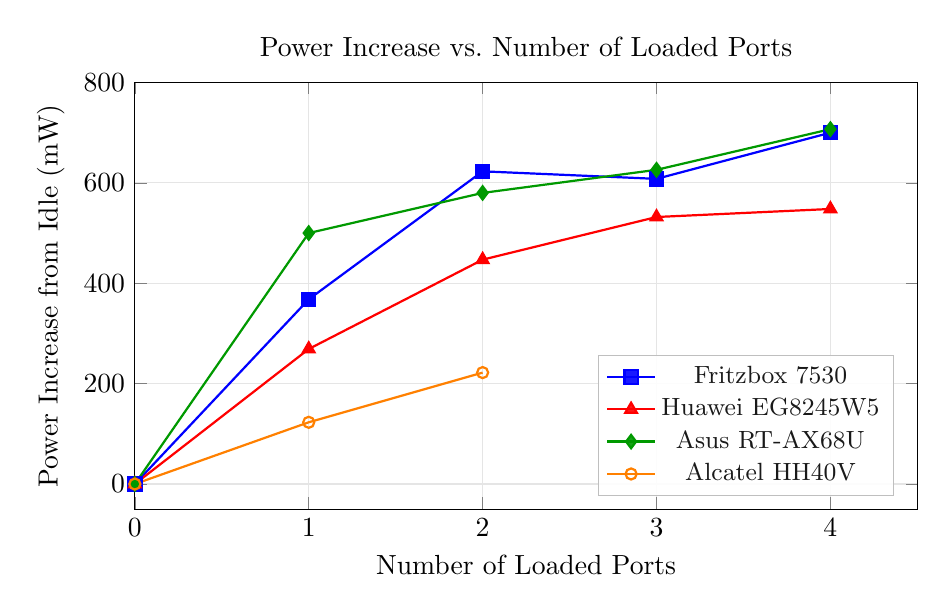
\begin{tikzpicture}
        \begin{axis}[
            width=0.95\linewidth,
            height=7cm,
            xlabel={Number of Loaded Ports},
            ylabel={Power Increase from Idle (mW)},
            xmin=0, xmax=4.5,
            ymin=-50, ymax=800,
            xtick={0,1,2,3,4},
            grid=major,
            grid style={gray!20},
            legend pos=south east,
            legend style={font=\small, fill=white, fill opacity=0.9, draw=gray!50},
            title={Power Increase vs.\ Number of Loaded Ports},
            mark options={scale=1.2},
        ]
            % Fritzbox: 0, +368, +623, +608, +700
            \addplot[blue, thick, mark=square*] coordinates {
                (0,0) (1,368) (2,623) (3,608) (4,700)
            };
            \addlegendentry{Fritzbox 7530}

            % Huawei: 0, +269, +447, +532, +548
            \addplot[red, thick, mark=triangle*] coordinates {
                (0,0) (1,269) (2,447) (3,532) (4,548)
            };
            \addlegendentry{Huawei EG8245W5}

            % Asus: 0, +500, +580, +626, +707
            \addplot[green!60!black, thick, mark=diamond*] coordinates {
                (0,0) (1,500) (2,580) (3,626) (4,707)
            };
            \addlegendentry{Asus RT-AX68U}

            % Alcatel: 0, +123, +222 (only 2 ports)
            \addplot[orange, thick, mark=o, mark options={solid, fill=orange}] coordinates {
                (0,0) (1,123) (2,222)
            };
            \addlegendentry{Alcatel HH40V}
        \end{axis}
    \end{tikzpicture}
    \caption{Power increase above idle baseline as a function of loaded port count. By plotting the delta from each device's idle power, all four devices become directly comparable regardless of their absolute power level. Note the Fritzbox's dip at 3~ports (CPU saturation reduces throughput and thus power). The Alcatel has only 2 ports.}
    \label{fig:power_delta_comparison}
\end{figure}

\paragraph{Key Findings for RQ1:}
\begin{itemize}
    \item All devices show a measurable power increase when ports are loaded, ranging from +222\,mW (Alcatel, 2~ports) to +707\,mW (Asus, 4~ports).
    \item The \textbf{Fritzbox~7530} exhibits a non-monotonic power profile: power peaks at 2~ports (5055\,mW) and then \emph{decreases} at 3~ports (5040\,mW). This is due to CPU saturation---the device cannot sustain full throughput on 3+ ports, so it does less total work and consumes slightly less power. This is a noteworthy finding: under CPU-bound conditions, adding more loaded ports can actually \emph{reduce} total power consumption because the bottleneck shifts from the PHY/switching fabric to the CPU.
    \item The \textbf{Huawei} and \textbf{Asus} devices show monotonically increasing power with near-linear throughput scaling, indicating their CPUs are not the bottleneck at 4$\times$1\,Gbps.
    \item The per-port power increment is small relative to idle power: approximately 30--175\,mW per additional loaded port, depending on the device.
\end{itemize}

% ===== RQ4 (Partial): Idle Power Suitability =====
\subsubsection{RQ4 (Partial): Idle Power and Continuous Operation Suitability}
\label{sec:rq4-results}

Table~\ref{tab:idle-power} presents the idle power measurements and estimated annual energy costs.

\begin{table}[H]
    \centering
    \caption{Idle power consumption ranking and estimated annual energy cost (at €0.25/kWh).}
    \label{tab:idle-power}
    \footnotesize
    \begin{tabular}{l r r r}
        \toprule
        \textbf{Device} & \textbf{Idle Power (W)} & \textbf{Annual Energy (kWh)} & \textbf{Annual Cost (€)} \\
        \midrule
        Alcatel HH40V       & 1.85 &  16.2 &  4.06 \\
        Fritzbox 7530       & 4.43 &  38.8 &  9.70 \\
        Asus RT-AX68U       & 8.23 &  72.1 & 18.01 \\
        Huawei EG8245W5-8T  & 8.96 &  78.5 & 19.63 \\
        \bottomrule
    \end{tabular}
\end{table}

\begin{figure}[H]
    \centering
    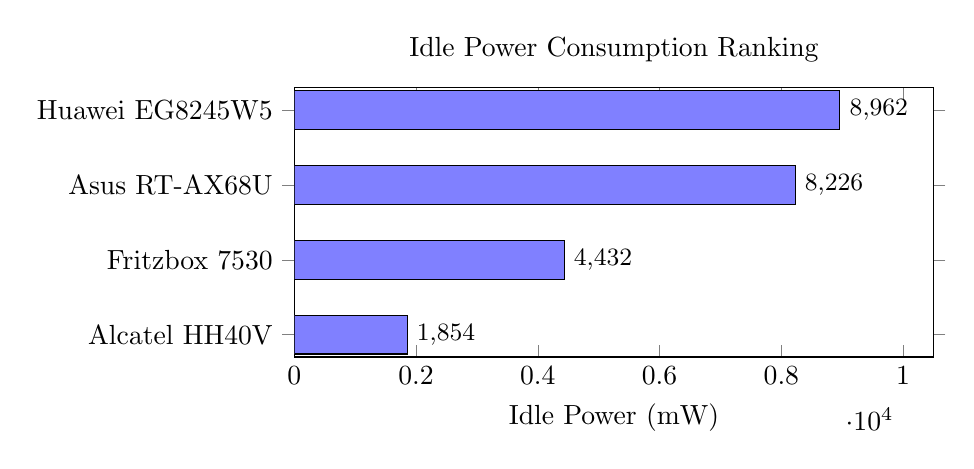
\begin{tikzpicture}
        \begin{axis}[
            xbar,
            width=0.80\textwidth,
            height=5cm,
            xlabel={Idle Power (mW)},
            symbolic y coords={Alcatel HH40V, Fritzbox 7530, Asus RT-AX68U, Huawei EG8245W5},
            ytick=data,
            nodes near coords,
            nodes near coords style={font=\small},
            xmin=0, xmax=10500,
            bar width=14pt,
            title={Idle Power Consumption Ranking},
        ]
            \addplot[fill=blue!50] coordinates {(1854,Alcatel HH40V) (4432,Fritzbox 7530) (8226,Asus RT-AX68U) (8962,Huawei EG8245W5)};
        \end{axis}
    \end{tikzpicture}
    \caption{Idle power ranking. The Alcatel draws less than half the power of the Fritzbox and less than a quarter of the Asus/Huawei devices.}
    \label{fig:idle_power_ranking}
\end{figure}

\paragraph{Key Findings for RQ4 (Partial):}
\begin{itemize}
    \item There is a 4.8$\times$ difference in idle power between the most efficient (Alcatel: 1.85\,W) and least efficient (Huawei: 8.96\,W) device.
    \item Annual idle energy costs range from €4 to nearly €20---a €16 difference that becomes significant in deployments with many access points.
    \item All four devices exceed the typical 2\,W standby threshold discussed in energy efficiency regulations, though the Alcatel is close. However, these are ``cables connected, idle'' measurements, not true standby (which would require disconnecting all Ethernet links and disabling Wi-Fi).
    \item \textbf{Limitation:} These are 10-minute idle measurements. A full 24-hour measurement (as planned for the complete RQ4 analysis) would capture any periodic background activity (firmware updates, Wi-Fi beaconing, DHCP renewal, etc.).
\end{itemize}

% ===== RQ8 (Partial): Rated vs Real Max =====
\subsubsection{RQ8 (Partial): Rated vs.\ Observed Maximum Power}
\label{sec:rq8-results}

Table~\ref{tab:rated-vs-real} compares the manufacturer's rated maximum power with the maximum power observed during the test.

\begin{table}[H]
    \centering
    \caption{Rated maximum vs.\ observed maximum power under full Ethernet load. The ``Utilization'' column indicates what fraction of the rated maximum was reached.}
    \label{tab:rated-vs-real}
    \footnotesize
    \begin{tabular}{l r r r r}
        \toprule
        \textbf{Device} & \textbf{Rated (W)} & \textbf{Observed (W)} & \textbf{Utilization} & \textbf{Headroom (W)} \\
        \midrule
        Fritzbox 7530       & 18 & 5.65 & 31.4\% & 12.35 \\
        Huawei EG8245W5-8T  & 24 & 9.58 & 39.9\% & 14.42 \\
        Asus RT-AX68U       & 33 & 9.22 & 27.9\% & 23.78 \\
        Alcatel HH40V       & 10 & 2.14 & 21.4\% & 7.86 \\
        \bottomrule
    \end{tabular}
\end{table}

\paragraph{Key Findings for RQ8 (Partial):}
\begin{itemize}
    \item None of the tested devices came close to their rated maximum power. The highest utilization was the Huawei at 39.9\% of its 24\,W rating.
    \item The rated maximum appears to account for \emph{all} subsystems operating simultaneously (Ethernet at full load \emph{plus} Wi-Fi radios active with clients \emph{plus} USB peripherals). Since this test only exercised Ethernet ports, significant power headroom remains.
    \item The \textbf{Asus RT-AX68U} has the largest gap: its 33\,W rating vs.\ 9.22\,W observed suggests that the Wi-Fi 6 radios (especially the 5\,GHz radio) likely account for a substantial portion of the rated maximum.
    \item \textbf{Limitation:} To fully answer RQ8, future tests should activate all subsystems simultaneously (Ethernet + Wi-Fi + USB) and attempt to reach the rated maximum.
\end{itemize}

% ---------------------------------------------------------------------------
\subsection{Measurement Considerations}
\label{sec:measurement-considerations}
% ---------------------------------------------------------------------------

Several factors should be considered when interpreting these results:

\begin{enumerate}
    \item \textbf{Power meter resolution:} The DECT~200 reports power in discrete steps of approximately 70\,mW. For devices where the load-induced power increase is small (e.g., Huawei: $\sim$550\,mW over 4~ports), the per-port incremental power ($\sim$137\,mW) is only about 2 discrete steps, limiting measurement precision for fine-grained per-port analysis.
    \item \textbf{CPU-targeted traffic:} All traffic was directed at the device's own IP, engaging the CPU stack rather than the hardware switching fabric. A Layer~2 forwarding test (e.g., port A$\rightarrow$B loopback) would likely show different power characteristics.
    \item \textbf{No zero-cable baseline:} The pre-test baseline had all cables physically connected (link up, no traffic). The power cost of merely maintaining a GbE link (PHY active, auto-negotiation) vs.\ having no cable connected was not isolated.
    \item \textbf{Throughput anomalies:} Some data points show transient throughput spikes (especially the Fritzbox and Alcatel) that exceed steady-state values. These are measurement artifacts caused by buffered packet bursts aligning with the 5-second polling window.
\end{enumerate}

% ---------------------------------------------------------------------------
\subsection{Summary of Findings}
\label{sec:results-summary}
% ---------------------------------------------------------------------------

Table~\ref{tab:results-summary} provides a comprehensive comparison of all key metrics across the four devices.

\begin{table}[H]
    \centering
    \caption{Comprehensive summary of Test~1 results across all four devices.}
    \label{tab:results-summary}
    \small
    \begin{tabular}{l r r r r}
        \toprule
        \textbf{Metric} & \textbf{Fritzbox} & \textbf{Huawei} & \textbf{Asus} & \textbf{Alcatel} \\
        \midrule
        Idle Power (mW)              & 4432  & 8962  & 8226  & 1854 \\
        Max Load Power (mW)          & 5132  & 9510  & 8933  & 2076 \\
        Power Increase (mW)          & +700  & +548  & +707  & +222 \\
        Power Increase (\%)          & 15.8  & 6.1   & 8.6   & 12.0 \\
        Max Throughput (Mbps)        & 2483  & 3815  & 3816  & 257 \\
        Theoretical Max (Mbps)       & 4000  & 4000  & 4000  & 200 \\
        Throughput Achieved (\%)     & 62.1  & 95.4  & 95.4  & 128.5\textsuperscript{*} \\
        Peak Efficiency (Mbps/W)     & 491   & 401   & 427   & 124 \\
        Rated Max (W)                & 18    & 24    & 33    & 10 \\
        Rated Utilization (\%)       & 31.4  & 39.9  & 27.9  & 21.4 \\
        \bottomrule
        \multicolumn{5}{l}{\textsuperscript{*}\scriptsize Measurement artifact: 5-second polling window captures burst averages above 200\,Mbps.} \\
    \end{tabular}
\end{table}

This concludes the analysis of Test~1. The remaining research questions (RQ2, RQ3, RQ5--RQ7, RQ9) require additional test setups as described in Section~\ref{sec:test-setups}.
\todo{Add results for Tests 2--5 as they are completed.}
